\section{Methodology}
\label{sec:methodology}

The common pipeline is divided into three blocks following the presentation
logic of the reference journal article. Each block has an explicit input,
transformation, output, and pseudocode. Figure~\ref{fig:pipeline} summarizes
their relationship.

% Full-width TikZ overview shared by the Elsevier and IEEE entry points.
\usetikzlibrary{arrows.meta,positioning}

\begin{figure*}[!t]
\centering
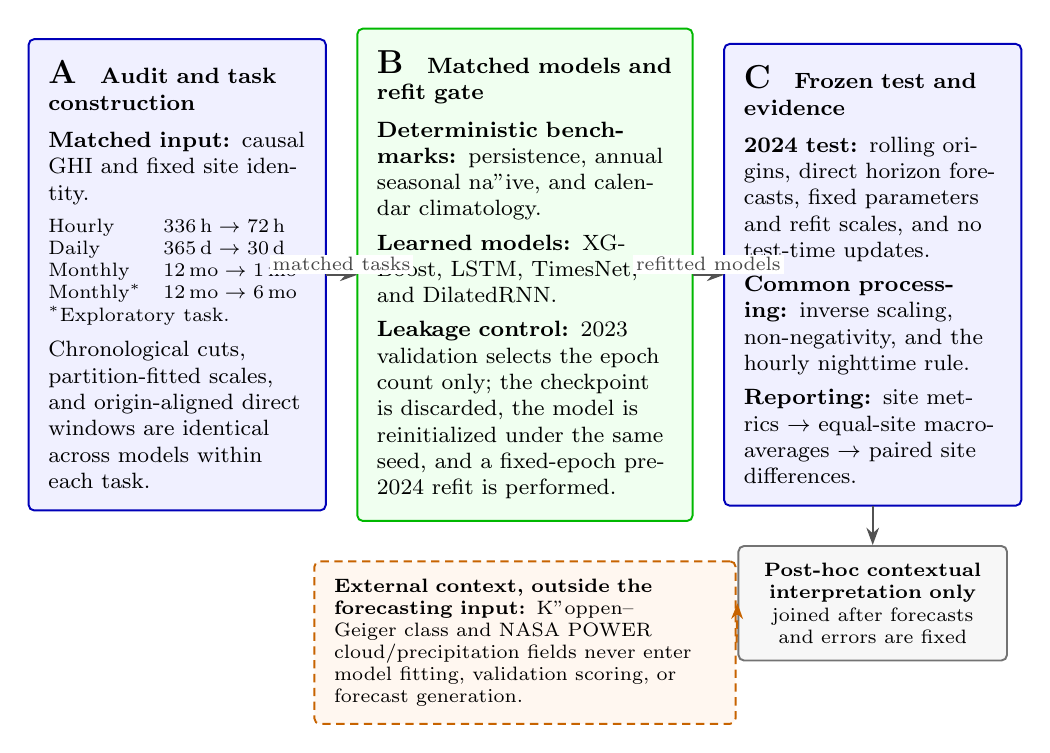
\begin{tikzpicture}[
  font=\footnotesize,
  stage/.style={
    draw=#1!72!black,
    fill=#1!6,
    rounded corners=2pt,
    line width=0.7pt,
    align=left,
    inner xsep=2.5mm,
    inner ysep=2.8mm,
    outer sep=0pt
  },
  flow arrow/.style={
    -{Stealth[length=2.2mm,width=1.6mm]},
    draw=black!68,
    line width=0.8pt
  },
  arrow label/.style={
    fill=white,
    inner sep=1pt,
    font=\scriptsize,
    text=black!72
  },
  external/.style={
    draw=orange!78!black,
    fill=orange!6,
    densely dashed,
    rounded corners=2pt,
    line width=0.7pt,
    align=left,
    inner xsep=2.5mm,
    inner ysep=2.2mm,
    font=\scriptsize
  },
  posthoc/.style={
    draw=black!55,
    fill=black!3,
    rounded corners=2pt,
    line width=0.7pt,
    align=center,
    inner xsep=2.5mm,
    inner ysep=2.2mm,
    font=\scriptsize
  }
]

\node[stage=blue,text width=0.27\textwidth] (stage-a) {
  {\large\bfseries A}\quad\textbf{Audit and task construction}\\[1.4mm]
  \textbf{Matched input:} causal GHI and fixed site identity.\\[1.2mm]
  {\scriptsize
  \begin{tabular}{@{}l@{\quad}l@{}}
    Hourly & $336\,\mathrm{h}\rightarrow72\,\mathrm{h}$ \\
    Daily & $365\,\mathrm{d}\rightarrow30\,\mathrm{d}$ \\
    Monthly & $12\,\mathrm{mo}\rightarrow1\,\mathrm{mo}$ \\
    Monthly$^{\ast}$ & $12\,\mathrm{mo}\rightarrow6\,\mathrm{mo}$
  \end{tabular}}\\[-0.2mm]
  {\scriptsize $^{\ast}$Exploratory task.}\\[1.2mm]
  Chronological cuts, partition-fitted scales, and origin-aligned direct
  windows are identical across models within each task.
};

\node[stage=green,text width=0.31\textwidth,right=4mm of stage-a] (stage-b) {
  {\large\bfseries B}\quad\textbf{Matched models and refit gate}\\[1.4mm]
  \textbf{Deterministic benchmarks:} persistence, annual seasonal na"ive,
  and calendar climatology.\\[1.0mm]
  \textbf{Learned models:} XGBoost, LSTM, TimesNet, and DilatedRNN.\\[1.0mm]
  \textbf{Leakage control:} 2023 validation selects the epoch count only;
  the checkpoint is discarded, the model is reinitialized under the same
  seed, and a fixed-epoch pre-2024 refit is performed.
};

\node[stage=blue,text width=0.27\textwidth,right=4mm of stage-b] (stage-c) {
  {\large\bfseries C}\quad\textbf{Frozen test and evidence}\\[1.4mm]
  \textbf{2024 test:} rolling origins, direct horizon forecasts, fixed
  parameters and refit scales, and no test-time updates.\\[1.0mm]
  \textbf{Common processing:} inverse scaling, non-negativity, and the hourly
  nighttime rule.\\[1.0mm]
  \textbf{Reporting:} site metrics $\rightarrow$ equal-site macro-averages
  $\rightarrow$ paired site differences.
};

\draw[flow arrow] (stage-a.east) --
  node[arrow label,above] {matched tasks} (stage-b.west);
\draw[flow arrow] (stage-b.east) --
  node[arrow label,above] {refitted models} (stage-c.west);

\node[external,text width=0.40\textwidth,below=5mm of stage-b] (external-data) {
  \textbf{External context, outside the forecasting input:}
  K"oppen--Geiger class and NASA POWER cloud/precipitation fields never enter
  model fitting, validation scoring, or forecast generation.
};

\node[posthoc,text width=0.24\textwidth,below=5mm of stage-c] (interpretation) {
  \textbf{Post-hoc contextual interpretation only}\\
  joined after forecasts and errors are fixed
};

\draw[flow arrow] (stage-c.south) -- (interpretation.north);
\draw[-{Stealth[length=2.0mm,width=1.5mm]},densely dashed,
      draw=orange!78!black,line width=0.75pt]
  (external-data.east) -- (interpretation.west);

\end{tikzpicture}
\caption{Unified multi-resolution pipeline. The four frozen task contracts are
evaluated on matched origins across deterministic benchmarks and learned
models. External climate and weather products are excluded from model inputs
and enter only after forecasts and errors are fixed. Algorithms~\ref{alg:block_a}--
\ref{alg:block_c} provide the corresponding pseudocode.}
\label{fig:pipeline}
\end{figure*}


\subsection{Block A: data preparation}

Block A converts audited NSRDB series into resolution-specific supervised
examples. All calculations for an origin $t$ use only values available before
or at that origin.

\begin{algorithm}[htbp]
\caption{Block A---data preparation and temporal windows}
\label{alg:block_a}
\begin{algorithmic}[1]
\Require Raw series, locations $\mathcal{L}$, resolution $r$, context $c$, horizon $h$
\Ensure Chronological training, validation, and test windows
\For{each location $\ell\in\mathcal{L}$}
  \State audit timestamps, missing values, duplicates, and invalid GHI
  \State aggregate GHI at resolution $r$
  \State split the series chronologically before fitting transformations
  \State fit scaling and derived-feature rules on training data only
  \State create $(c,h)$ windows without crossing partition boundaries
\EndFor
\end{algorithmic}
\end{algorithm}

The output of Block A is a set of origin-aligned samples shared by every model
within the same experiment. This prevents changes in sample availability from
being mistaken for architectural gains.

\subsection{Block B: model development and forecasting}

\begin{algorithm}[htbp]
\caption{Block B---matched training and forecasting}
\label{alg:block_b}
\begin{algorithmic}[1]
\Require Training and validation windows, predefined model search spaces
\Ensure Fixed models and raw forecasts for every test origin
\For{each model $m\in\{\text{TimesNet},\text{DilatedRNN},\text{baselines}\}$}
  \State select hyperparameters using validation data only
  \State reinitialize and refit the selected configuration on pre-test data
  \For{each chronological test origin}
    \State predict the complete horizon without future target information
  \EndFor
\EndFor
\end{algorithmic}
\end{algorithm}

TimesNet and DilatedRNN will be trained with the same samples and forecast
origins at each shared resolution. Architecture-specific context lengths may
be studied as an ablation, but the primary comparison will keep the available
information equivalent.

\subsection{Block C: physical post-processing and evaluation}

\begin{algorithm}[htbp]
\caption{Block C---post-processing, metrics, and case selection}
\label{alg:block_c}
\begin{algorithmic}[1]
\Require Raw forecasts, reference targets, location metadata
\Ensure Aggregate, local, horizon-wise, and adverse-case results
\State invert training-fitted transformations
\State apply the same non-negativity rule to every eligible model
\State apply the documented solar-elevation rule to hourly forecasts
\State compute every metric first by location and then its macro-average
\State rank models under the declared primary metric
\State select favorable and unfavorable cases using a rule fixed in advance
\end{algorithmic}
\end{algorithm}

The favorable and unfavorable examples are selected after computing all
location--origin errors, but the selection rule must be declared before their
interpretation. A weather case will be labeled rainy or cloudy only when an
independent meteorological field or source confirms that condition.

